% !TeX program = xelatex
% 正文来源：../tex/金融经济学_王江/12_均值方差偏好.tex、13_CAPM.tex、14_APT.tex。
% 版式来源：同目录 ESG与碳风险定价_文献综述汇报.tex。
% 在本目录运行 latexmk -xelatex 第12—14讲_均值方差偏好_CAPM与APT.tex。

\documentclass[UTF8,fontset=none,aspectratio=169,10pt]{ctexbeamer}
\DeclareFontShape{OT1}{cmr}{m}{n}{%
  <-6>cmr5 <6-7>cmr6 <7-8>cmr7 <8-9>cmr8 <9-10>cmr9
  <10-12>cmr10 <12-17>cmr12 <17->cmr17}{}
\usepackage{njust_beamer}
\AtBeginSection[]{}
\usepackage{amsmath,amssymb,booktabs,tabularx,array,graphicx,adjustbox}
\usetikzlibrary{arrows.meta,positioning,calc}
\definecolor{ink}{RGB}{24,49,65}
\definecolor{accent}{RGB}{31,83,145}
\definecolor{accentlight}{RGB}{226,235,247}
\definecolor{gold}{RGB}{190,126,35}
\definecolor{risk}{RGB}{147,53,52}
\definecolor{muted}{RGB}{93,108,117}
\setbeamercolor{normal text}{fg=ink,bg=white}
\setbeamercolor{structure}{fg=accent}
\setbeamercolor{frametitle}{fg=ink,bg=white}
\setbeamercolor{block title}{fg=white,bg=accent}
\setbeamercolor{block body}{fg=ink,bg=accentlight}
\setbeamercolor{alerted text}{fg=risk}
\setbeamertemplate{navigation symbols}{}
\setbeamertemplate{itemize item}{\color{accent}\small$\blacktriangleright$}
\setbeamertemplate{itemize subitem}{\color{gold}\scriptsize$\blacktriangleright$}
\setbeamertemplate{blocks}[rounded][shadow=false]
\setlength{\parskip}{0.30em}
\setlength{\tabcolsep}{5pt}
\renewcommand{\arraystretch}{1.28}
\newcolumntype{Y}{>{\raggedright\arraybackslash}X}
\newcolumntype{P}[1]{>{\raggedright\arraybackslash}p{#1}}
\renewcommand{\tabularxcolumn}[1]{p{#1}}
% 保持原主题标题位置，仅在存在副标题时显示分隔线。
\makeatletter
\setbeamertemplate{frametitle}{%
  \begin{beamercolorbox}[wd=\paperwidth,ht=2.0ex,dp=.2ex,leftskip=10pt]{}
    \usebeamerfont{frametitle}\usebeamercolor[fg]{frametitle}\insertframetitle
    \ifx\insertframesubtitle\@empty\else
      ~\textcolor{njustpurple2!50}{\rule[-.2ex]{.08em}{1.8ex}}~
      \usebeamerfont{framesubtitle}\usebeamercolor[fg]{framesubtitle}\insertframesubtitle
    \fi
  \end{beamercolorbox}%
}
\makeatother
\newcommand{\source}[1]{%
  \begin{tikzpicture}[remember picture,overlay]
    \node[anchor=south west,inner sep=0pt,text width=.91\paperwidth,
      align=left,font=\tiny,text=muted]
    at ([xshift=.035\paperwidth,yshift=.68cm]current page.south west)
      {讲义来源：#1};
  \end{tikzpicture}%
}
\newcommand{\lead}[1]{{\color{accent}\bfseries #1}\par\vspace{0.10cm}}
\newcommand{\spaceditems}{\setlength{\itemsep}{0.22cm}}
\newcommand{\keyline}[1]{%
  \begin{beamercolorbox}[wd=\linewidth,sep=0.16cm,rounded=true]{block body}
    \centering\bfseries #1
  \end{beamercolorbox}
}
% 参考文献按 GB/T 7714—2025 顺序编码制著录。
\newenvironment{gbreferences}[1]{%
  \setbeamertemplate{enumerate item}{[\insertenumlabel]}
  \setbeamercolor{enumerate item}{fg=ink}
  \begin{enumerate}\setcounter{enumi}{#1}\setlength{\itemsep}{.18cm}
}{\end{enumerate}}

% 由主题绘制页眉和底部进度条。
\newcommand{\lecturechapter}{12}
\setbeamertemplate{footline}[progress bar]
% 首次编译尚无 .nav 文件时，给主题提供非零帧数，避免累乘溢出。
\renewcommand{\inserttotalframenumber}{\number\numexpr\value{framenumber}+1\relax}
\newcommand{\study}[1]{\framesubtitle{\small #1}}
\newcommand{\bodygap}{\par\vspace{.20cm}}

% 内容框沿用讲义的边框、底色和标题样式。
% 讲义与 Beamer 共用的知识、例题和小结等内容框。
\tcbset{
    four three one box/.style={
        enhanced,
        breakable,
        parbox=false,
        boxrule=0.4pt,
        leftrule=1.4pt,
        arc=2pt,
        left=7pt,
        right=7pt,
        top=5pt,
        bottom=5pt,
        before skip=.5em plus .2em minus .1em,
        after skip=.5em plus .2em minus .1em,
        before upper=\indent,
        fonttitle=\bfseries
    },
    knowledge/.style={
        four three one box,
        colback=blue!2!white,
        colframe=blue!55!black,
        colbacktitle=blue!8!white,
        coltitle=blue!60!black
    },
    warning/.style={
        four three one box,
        colback=red!2!white,
        colframe=red!60!black,
        colbacktitle=red!8!white,
        coltitle=red!65!black
    },
    example/.style={
        four three one box,
        colback=teal!2!white,
        colframe=teal!55!black,
        colbacktitle=teal!8!white,
        coltitle=teal!60!black
    },
    practice/.style={
        four three one box,
        colback=violet!2!white,
        colframe=violet!55!black,
        colbacktitle=violet!8!white,
        coltitle=violet!60!black
    },
    summary/.style={
        four three one box,
        colback=black!1!white,
        colframe=black!45,
        colbacktitle=black!7!white,
        coltitle=black!70
    }
}


% 本讲内部编号沿用讲义。跨讲及课后习题引用保留讲义中的编号。
\renewcommand{\theequation}{\lecturechapter.\arabic{equation}}
\renewcommand{\theHequation}{\lecturechapter.\arabic{equation}}
\newcounter{wjTwelveTheorem}
\newcounter{wjTwelveCorollary}
\newcounter{wjTwelveFigure}
\renewcommand{\thewjTwelveTheorem}{12.\arabic{wjTwelveTheorem}}
\renewcommand{\thewjTwelveCorollary}{12.\arabic{wjTwelveCorollary}}
\renewcommand{\thewjTwelveFigure}{12.\arabic{wjTwelveFigure}}
\newcommand{\WJTwelveTheorem}[1]{\refstepcounter{wjTwelveTheorem}\label{#1}\textbf{定理 \thewjTwelveTheorem}\quad}
\newcommand{\WJTwelveCorollary}[1]{\refstepcounter{wjTwelveCorollary}\label{#1}\textbf{推论 \thewjTwelveCorollary}\quad}
\newcommand{\WJInputFigure}[2][.64\textheight]{%
  \resizebox{!}{#1}{\input{../tex/金融经济学_王江/figures/#2.tex}}%
}

% The handout body is paginated by sync-chapter12.py without rewriting its text.
\newcommand{\WJTwelveFigureStart}[1]{\refstepcounter{wjTwelveFigure}\label{#1}}
\newcommand{\WJTwelveFigureCaption}[1]{\par\smallskip 图\thewjTwelveFigure\quad #1}
\newcounter{wjFigure}
\newcommand{\WJFigureStart}[1]{\refstepcounter{wjFigure}\label{#1}}
\newcommand{\WJFigureCaption}[1]{\par\smallskip 图\thewjFigure\quad #1}
\newcounter{wjTwelveExercise}
\renewcommand{\thewjTwelveExercise}{12.\arabic{wjTwelveExercise}}
\newcommand{\WJTwelveExercise}[2]{%
  \refstepcounter{wjTwelveExercise}\label{#1}\textbf{\thewjTwelveExercise#2}\quad}
\colorlet{WJReferenceColor}{accent}

% References to chapters outside this deck retain their handout numbers.
\newcommand{\WJOutsideReference}[2]{\expandafter\def\csname wjoutside:#1\endcsname{#2}}
\WJOutsideReference{chap:wj-two}{二}
\WJOutsideReference{chap:wj-eleven}{十一}
\WJOutsideReference{axiom:wj-two-1}{1}
\WJOutsideReference{def:wj-two-6}{2.6}
\WJOutsideReference{def:wj-nine-4}{9.4}
\WJOutsideReference{eq:wj-six-4}{6.4}
\WJOutsideReference{eq:wj-seven-2}{7.2}
\WJOutsideReference{eq:wj-8-8}{8.8}
\WJOutsideReference{eq:wj-8-9}{8.9}
\WJOutsideReference{exer:wj-eight-3}{8.3}
\WJOutsideReference{exer:wj-nine-7}{9.7}
\WJOutsideReference{sec:wj-nine-2}{9.2}
\WJOutsideReference{thm:wj-nine-4}{9.4}
\WJOutsideReference{thm:wj-nine-6}{9.6}
\NewDocumentCommand{\WJRef}{m m O{}}{%
  \ifcsname wjoutside:#1\endcsname
    #2\csname wjoutside:#1\endcsname#3%
  \else
    \hyperref[#1]{#2\ref*{#1}#3}%
  \fi}
\NewDocumentCommand{\WJEqRef}{m m O{}}{%
  \ifcsname wjoutside:#1\endcsname
    #2(\csname wjoutside:#1\endcsname)#3%
  \else
    \hyperref[#1]{#2(\ref*{#1})#3}%
  \fi}
\newcommand{\WJLink}[2]{%
  \ifcsname wjoutside:#1\endcsname #2\else\hyperref[#1]{#2}\fi}

\pgfkeys{
  /wj slide solution/.cd,
  label-content/.store in=\wjSlideSolutionLabel,
  .unknown/.code={}
}
\makeatletter
\newenvironment{WJFullChapterSlides}{%
  % Preserve starred references when amsmath writes a custom equation tag.
  \let\ref\beamer@origref%
  \def\WJHandoutKnowledge{}%
  \def\thechapter{\lecturechapter}%
  % Beamer collects a frame before splitting it, so give long boxes a slide-sized break target.
  \tcbset{break at=.80\textheight/.80\textheight/.80\textheight/.80\textheight}%
  \providecommand{\Needspace}[1]{}%
  \renewcommand{\Needspace}[1]{}%
  % Inline notes stay with the paragraph on continued frames.
  \RenewDocumentCommand{\footnote}{m}{\space{\footnotesize（注：##1）}}%
  \renewcommand{\qedhere}{}%
  \DeclareDocumentEnvironment{solution}{O{}}{%
    \par\smallskip
    \pgfkeys{/wj slide solution/.cd,label-content={解答},##1}%
    \ifx\wjSlideSolutionLabel\empty\else
      \noindent\textbf{\wjSlideSolutionLabel}\quad
    \fi
  }{\par\smallskip}%
  \let\wjSlideEnumerate\enumerate
  \let\wjSlideEndEnumerate\endenumerate
  \RenewDocumentEnvironment{enumerate}{o}{%
    \IfNoValueTF{##1}{\wjSlideEnumerate}{%
      \ifstrequal{##1}{label=(\alph*)}{\wjSlideEnumerate[(a)]}{%
        \ifstrequal{##1}{label=(\arabic*)}{\wjSlideEnumerate[(1)]}{\wjSlideEnumerate[##1]}%
      }%
    }%
  }{\wjSlideEndEnumerate}%
  \renewcommand{\WJInputFigure}[2][.46\textheight]{%
    \begin{adjustbox}{max width=\linewidth,max height=##1}%
      \input{../tex/金融经济学_王江/figures/##2.tex}%
    \end{adjustbox}%
  }%
}{}
\makeatother

\newcommand{\WJFeasibleDirectionFrame}{%
\begin{frame}[t]{一阶条件为什么给出最小值}
令 $z_p+h$ 为任意另一组可行权重。两条约束保持不变，所以 $h^{\mathsf T}\iota=h^{\mathsf T}\bar r=0$。直接展开目标函数：
\[
 f(z_p+h)-f(z_p)
 =\underbrace{h^{\mathsf T}\Sigma z_p}_{=\,\lambda_r h^{\mathsf T}\bar r+\lambda_1 h^{\mathsf T}\iota=0}
  +\underbrace{\tfrac12 h^{\mathsf T}\Sigma h}_{>0\ \text{若}\ h\ne0}.
\]
任何其他可行权重的方差都更高，因此 $z_p$ 是唯一的全局最小值。

本节允许卖空，沿满足等式约束的方向可以双向移动。若加上 $z_i\ge0$，零权重会限制可行方向，边界上的最优解要结合可行方向或 KKT 条件判断。
\end{frame}
}

\newcounter{wjThirteenTheorem}
\newcounter{wjThirteenExample}
\newcounter{wjThirteenFigure}
\renewcommand{\thewjThirteenTheorem}{13.\arabic{wjThirteenTheorem}}
\renewcommand{\thewjThirteenExample}{13.\arabic{wjThirteenExample}}
\renewcommand{\thewjThirteenFigure}{13.\arabic{wjThirteenFigure}}
\newcommand{\WJThirteenTheorem}[1]{\refstepcounter{wjThirteenTheorem}\label{#1}\textbf{定理 \thewjThirteenTheorem}\quad}
\newcommand{\WJThirteenExample}[1]{\refstepcounter{wjThirteenExample}\label{#1}\textbf{例 \thewjThirteenExample}\quad}
\newcommand{\WJThirteenFigureStart}[1]{\refstepcounter{wjThirteenFigure}\label{#1}}
\newcommand{\WJThirteenFigureCaption}[1]{\par\smallskip 图\thewjThirteenFigure\quad #1}
\newcommand{\WJThirteenFigure}[2]{\WJThirteenFigureStart{#1}\WJThirteenFigureCaption{#2}}
\newcommand{\WJInputCaptionedFigure}[1]{%
  {\centering
  \resizebox*{!}{.74\textheight}{%
    \begin{minipage}{\linewidth}
      \input{../tex/金融经济学_王江/figures/#1.tex}%
    \end{minipage}%
  }\par}%
}

\newcounter{wjFourteenTheorem}
\renewcommand{\thewjFourteenTheorem}{14.\arabic{wjFourteenTheorem}}
\newcounter{wjFourteenLemma}
\renewcommand{\thewjFourteenLemma}{14.\arabic{wjFourteenLemma}}
\newcounter{wjFourteenDefinition}
\renewcommand{\thewjFourteenDefinition}{14.\arabic{wjFourteenDefinition}}
\newcommand{\WJFourteenTheorem}[1]{\refstepcounter{wjFourteenTheorem}\label{#1}\textbf{定理 \thewjFourteenTheorem}\quad}
\newcommand{\WJFourteenLemma}[1]{\refstepcounter{wjFourteenLemma}\label{#1}\textbf{引理 \thewjFourteenLemma}\quad}
\newcommand{\WJFourteenDefinition}[1]{\refstepcounter{wjFourteenDefinition}\label{#1}\textbf{定义 \thewjFourteenDefinition}\quad}
\newcounter{wjFourteenFigure}
\renewcommand{\thewjFourteenFigure}{14.\arabic{wjFourteenFigure}}
\newcommand{\WJFourteenFigureStart}[1]{\refstepcounter{wjFourteenFigure}\label{#1}}
\newcommand{\WJFourteenFigureCaption}[1]{\par\smallskip 图\thewjFourteenFigure\quad #1}
\newcommand{\WJFourteenFigure}[2]{\WJFourteenFigureStart{#1}\WJFourteenFigureCaption{#2}}

\newcommand{\LectureCover}{%
\begin{frame}[plain]
\begin{tikzpicture}[remember picture,overlay]
\node[anchor=south west,inner sep=0pt] at (current page.south west)
 {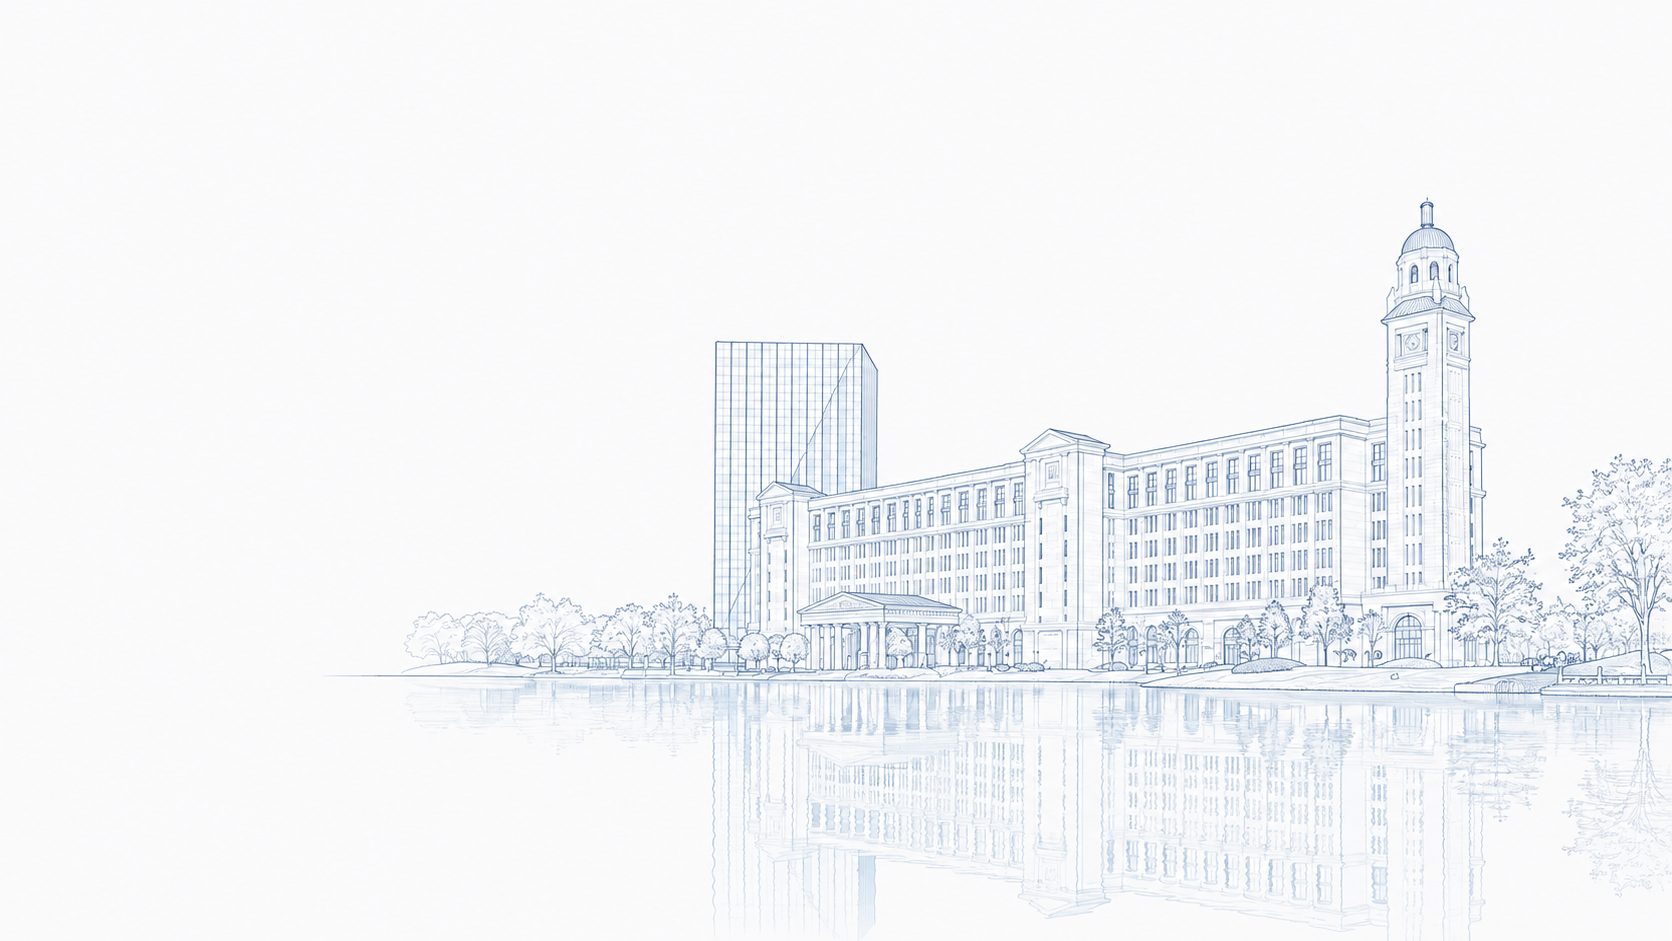
\includegraphics[width=\paperwidth,height=\paperheight]{cover_background.png}};
\node[anchor=north west,text=accent,font=\songti\bfseries\large]
 at ([xshift=.065\paperwidth,yshift=-.065\paperheight]current page.north west) {\insertshortauthor\quad\insertdate};
\node[anchor=north west,text=accent,font=\songti\bfseries]
 at ([xshift=.065\paperwidth,yshift=-.205\paperheight]current page.north west)
 {\fontsize{25}{32}\selectfont \inserttitle};
\draw[accent,line width=1.3pt] ([xshift=.065\paperwidth,yshift=-.43\paperheight]current page.north west)--([xshift=.58\paperwidth,yshift=-.43\paperheight]current page.north west);
\draw[accent,line width=3.4pt] ([xshift=.065\paperwidth,yshift=-.43\paperheight]current page.north west)--([xshift=.14\paperwidth,yshift=-.43\paperheight]current page.north west);
\node[anchor=north west,text=accent,font=\songti\large]
 at ([xshift=.065\paperwidth,yshift=-.465\paperheight]current page.north west)
 {\insertsubtitle};
\node[anchor=south west,text=accent,font=\songti\normalsize]
 at ([xshift=.065\paperwidth,yshift=.115\paperheight]current page.south west)
 {\insertauthor};
\end{tikzpicture}
\end{frame}
}

\author[金融经济学]{王江《金融经济学》}
\hypersetup{pdftitle={金融经济学第12—14讲：均值–方差偏好、CAPM与APT}}

\begin{document}

\part{第 12 讲 在均值--方差偏好下的投资组合选择}
\title[在均值--方差偏好下的投资组合选择]{%
  \shortstack[l]{在均值--方差偏好下的\\[-1pt]投资组合选择}}
\subtitle{前沿组合、基金分离与切点组合}
\date{第 12 讲}
\LectureCover

\begin{frame}[t]{本讲内容}
均值--方差偏好使参与者根据未来财富的均值和方差选择投资组合。本章先说明这种表示成立的条件，再求解最小方差问题，研究基金分离、有效前沿及证券与前沿组合之间的收益关系。
\bodygap
\begingroup
\renewcommand{\arraystretch}{1.28}
\begin{tabularx}{\textwidth}{@{}>{\color{accent}\bfseries}l Y@{}}
01 & \hyperref[sec:wj-twelve-1]{\textbf{均值--方差偏好}}\\
02 & \hyperref[sec:wj-twelve-2]{\textbf{均值--方差前沿组合}}\\
03 & \hyperref[sec:wj-twelve-3]{\textbf{均值--方差前沿组合的性质}}\\
04 & \hyperref[sec:wj-twelve-4]{\textbf{存在无风险资产的情形}}\\
05 & \hyperref[sec:wj-twelve-review]{\textbf{补充证明与练习}}\\
\end{tabularx}
\endgroup
\vfill\source{王江《金融经济学》第 12 章，印刷页 179--194。}
\end{frame}

\begin{WJFullChapterSlides}
\input{build/chapter12-full.tex}
\end{WJFullChapterSlides}

\renewcommand{\lecturechapter}{13}
\setcounter{equation}{0}
\part{第 13 讲 资本资产定价模型}
\title[资本资产定价模型]{资本资产定价模型}
\subtitle{市场组合、贝塔定价与均衡推导}
\date{第 13 讲}
\LectureCover


\begin{frame}[t]{本讲内容}
上一讲从个人选择得到有效组合及其贝塔关系。本章加入证券供给和市场出清，将有效风险组合识别为市场组合，从而得到资本资产定价模型（CAPM）。最后分别从二次效用和正态支付出发，展开这一均衡定价关系的推导。
\bodygap
\begingroup
\renewcommand{\arraystretch}{1.28}
\begin{tabularx}{\textwidth}{@{}>{\color{accent}\bfseries}l Y@{}}
01 & \hyperref[sec:wj-thirteen-1]{\textbf{市场组合}}\\
02 & \hyperref[sec:wj-thirteen-2]{\textbf{市场均衡}}\\
03 & \hyperref[sec:wj-thirteen-3]{\textbf{CAPM给出的资产定价关系}}\\
04 & \hyperref[sec:wj-thirteen-4]{\textbf{不存在无风险资产的CAPM}}\\
05 & \hyperref[sec:wj-thirteen-5]{\textbf{作为均衡结果的CAPM}}\\
\end{tabularx}
\endgroup
\vfill\source{王江《金融经济学》第 13 章，印刷页 197--211。}
\end{frame}

\section{市场组合}\label{sec:wj-thirteen-1}

\subsection{总持仓与市场价值权重}

\begin{frame}[t]{市场组合的总持仓与市值权重}
证券 $n$ 的总供给为 $\bar\theta_n$，价格为 $P_n$。全部风险证券的总供给本身构成\textbf{市场组合}，其总持仓向量为
\begin{equation}
 \theta_M=(\bar\theta_1,\ldots,\bar\theta_N)^{\mathsf T}.
 \label{eq:wj-13-1}
\end{equation}

在证券市场经济中，个人未来禀赋来自初始证券持仓。当市场没有无风险证券，或无风险证券的净供给为零时，未来总禀赋就等于风险证券市场组合的支付。市场组合可用证券数量表示，也可用投资价值权重表示。

\begin{tcolorbox}[knowledge,breakable=false]
令 $v_n=P_n\bar\theta_n$ 为证券 $n$ 的市场价值，$v_M=P^{\mathsf T}\theta_M=\sum_n v_n>0$ 为全部风险证券的总市值，则市场组合的权重为
\begin{equation}
 z_{n,M}=\frac{P_n\bar\theta_n}{v_M},\qquad
 z_M=(z_{1,M},\ldots,z_{N,M})^{\mathsf T},\quad\iota^{\mathsf T}z_M=1.
 \label{eq:wj-13-2}
\end{equation}
\end{tcolorbox}
\end{frame}

\begin{frame}[t]{市场组合的收益率}
其中 $\iota$ 为元素全为 $1$ 的列向量。总持仓 $\theta_M$ 描述证券的供给数量，价值权重 $z_M$ 描述每单位市场投资分配到各证券的比例。记 $\widetilde X$ 为风险证券的单位到期支付列向量。在各证券价格非零时，令 $\widetilde r_n=\widetilde X_n/P_n-1$，则市场组合的净收益率可写成
\[
 \widetilde r_M=\frac{\theta_M^{\mathsf T}\widetilde X}{v_M}-1
 =\sum_n z_{n,M}\widetilde r_n.
\]

第一种写法从市场总支付和总市值出发，第二种按市值权重加总各证券的净收益率。市场组合覆盖模型中的全部可交易风险证券，指数基金对它的近似程度取决于指数的资产覆盖与权重。
\end{frame}

\section{市场均衡}\label{sec:wj-thirteen-2}

\subsection{切点组合需求与市场出清}

\begin{frame}[t]{切点组合需求与市场出清}
先考虑存在无风险证券的情形。沿用第~\hyperref[sec:wj-twelve-4]{12.4}~节的共同信念、均值--方差偏好及自由借贷、卖空条件，假定个人最优解存在，且正超额收益的\hyperlink{wj-tangency-portfolio}{切点组合}存在。由式~\eqref{eq:wj-12-8}，参与者 $k$ 的风险权重向量为 $\alpha_k z_T$，其中 $\alpha_k$ 是风险证券的总投资比例。若个人投资财富为 $w_k$，则风险投资金额为 $A_k=w_k\alpha_k$，各只风险证券的需求金额为 $A_k z_T$，无风险证券的需求金额为 $w_k-A_k$。设无风险证券净供给为零，分别按市场价值加总两类需求，得到出清条件
\[
 \underbrace{\sum_k A_kz_T=v_Mz_M}_{\text{各风险证券按市场价值出清}},\qquad
 \underbrace{\sum_k(w_k-A_k)=0}_{\text{无风险证券净供给为零}}.
\]

总投资财富等于全部资产市值，即 $\sum_kw_k=v_M$，所以第二式给出 $\sum_kA_k=v_M$。
\end{frame}

\begin{frame}[t]{均衡市场组合等于切点组合}
\begin{tcolorbox}[knowledge,breakable=false]
\WJThirteenTheorem{thm:wj-thirteen-1} 在上述均值--方差经济中，市场达到均衡时，市场组合就是切点组合：$z_M=z_T$。
\end{tcolorbox}

\textbf{证明：}将 $\sum_kA_k=v_M$ 代入风险资产出清条件，得 $v_Mz_T=v_Mz_M$。由于 $v_M>0$，两边相除即得结论。\hfill$\square$
\end{frame}

\subsection{市场组合的有效性}

\begin{frame}[t]{市场组合的有效性}
市场组合因此位于有效前沿。个人最优投资可以写成无风险证券与市场组合的配置，个人风险承受能力决定风险投资的金额。原本需要估计最优风险权重的问题，在均衡中转化为观察各证券的市场价值权重；这也为持有广泛市场组合的指数投资提供了理论依据。
\end{frame}

\section[贝塔定价]{CAPM给出的资产定价关系}\label{sec:wj-thirteen-3}

\subsection{市场贝塔与证券市场线}

\begin{frame}[t]{CAPM 的市场贝塔关系}
\begin{tcolorbox}[knowledge,breakable=false]
\WJThirteenTheorem{thm:wj-thirteen-2} 若市场组合方差 $\sigma_M^2>0$，则对价格非零的任意证券 $n$，CAPM均衡满足
\begin{equation}
 \bar r_n-r_F
 =\underbrace{\beta_{n,M}}_{\text{市场贝塔}}\quad
  \underbrace{(\bar r_M-r_F)}_{\text{基准收益差}},\qquad
 \beta_{n,M}=\frac{\operatorname{Cov}(\widetilde r_n,\widetilde r_M)}{\sigma_M^2}.
 \label{eq:wj-13-3}
\end{equation}
\end{tcolorbox}

\textbf{证明：}由定理~\ref{thm:wj-thirteen-1}（均衡市场组合等于切点组合），$M=T$。将其代入上一讲的切点组合关系~\eqref{eq:wj-12-10}（组合风险溢价等于其切点贝塔乘以切点组合风险溢价），即得式~\eqref{eq:wj-13-3}。\hfill$\square$

证券的风险溢价等于其市场贝塔乘以市场风险溢价。贝塔衡量证券对市场组合风险的贡献，$\bar r_M-r_F$ 是每单位市场贝塔的风险价格；市场组合自身的贝塔为1。
\end{frame}

\begin{frame}[t]{证券市场线与消费贝塔关系}
第十讲式~(10.23) 对代表性参与者的边际效用作一阶展开，由此得到以总消费组合为基准的近似贝塔关系。当市场组合的支付等于总消费时，两讲的贝塔使用同一个基准组合。本讲从均值--方差最优性与市场出清直接得到式~\eqref{eq:wj-13-3}，它在上述均衡条件下精确成立。

以市场贝塔为横轴、期望收益率为纵轴，式~\eqref{eq:wj-13-3} 给出截距为 $r_F$、斜率为 $\bar r_M-r_F$ 的\textbf{证券市场线}（SML）。若纵轴改为风险溢价，SML经过原点。\hyperlink{wj-capital-market-line}{CML}则以总标准差为横轴，刻画有效组合；二者分别见图~\ref{fig:wj-thirteen-1}。
\end{frame}

\begin{frame}[t]{资本市场线与证券市场线}
\WJInputCaptionedFigure{13_CML与SML}
\vfill\source{王江《金融经济学》图 13.1，印刷页 201，沿用讲义图。}
\end{frame}

\subsection[系统风险与市场回归]{系统风险、剩余风险与市场回归}

\begin{frame}[t]{市场回归及其截距与斜率}
当市场收益方差为正时，可以将证券超额收益率对市场超额收益率作含截距的总体线性回归：
\begin{equation}
 \widetilde r_n-r_F=\alpha_n+\beta_{n,M}(\widetilde r_M-r_F)+\widetilde\varepsilon_n,
 \qquad \mathrm E[\widetilde\varepsilon_n]=0,
 \quad\operatorname{Cov}(\widetilde\varepsilon_n,\widetilde r_M)=0.
 \label{eq:wj-13-4}
\end{equation}

回归选择截距和斜率，使残差平方的期望最小。对截距求导得 $\mathrm E[\widetilde\varepsilon_n]=0$，对斜率求导得 $\mathrm E[\widetilde\varepsilon_n(\widetilde r_M-r_F)]=0$。两式合起来说明残差与市场收益的协方差为零。对式~\eqref{eq:wj-13-4} 两侧与市场收益取协方差，得到 $\operatorname{Cov}(\widetilde r_n,\widetilde r_M)=\beta_{n,M}\sigma_M^2$，所以回归斜率就是市场贝塔。再取期望得 $\alpha_n=\bar r_n-r_F-\beta_{n,M}(\bar r_M-r_F)$。由 CAPM 的期望收益关系~\eqref{eq:wj-13-3}，总体回归截距 $\alpha_n=0$，即资产的期望超额收益全部由市场贝塔项解释。
\end{frame}

\begin{frame}[t]{系统风险与剩余风险}
\begin{tcolorbox}[knowledge,breakable=false]
对式~\eqref{eq:wj-13-4} 取方差。由于市场收益与残差的协方差为零，资产收益的总风险可分为\textbf{系统风险}和\textbf{剩余风险}（非系统风险）：
\[
 \sigma_n^2=\underbrace{\beta_{n,M}^2\sigma_M^2}_{\text{系统风险方差}}
 +\underbrace{\sigma_{\varepsilon_n}^2}_{\text{剩余风险方差}}.
\]
当 $\sigma_n^2>0$ 时，市场回归的决定系数为
\[
 R_n^2=\frac{\beta_{n,M}^2\sigma_M^2}{\sigma_n^2}.
\]
\end{tcolorbox}

方差分解使用贝塔的平方，反映系统风险在总方差中的比重。CAPM 的风险溢价只补偿市场风险，并保留贝塔的符号。正贝塔资产与市场的协方差为正，负贝塔资产与市场负相关，具有对冲作用。不同证券的剩余收益仍可能彼此相关，剩余风险能分散多少取决于这些相关性。
\end{frame}

\begin{frame}[t]{例题}
\study{风险溢价、期望收益与风险构成}
\begin{tcolorbox}[example]
\WJThirteenExample{example:wj-thirteen-1} 资产 $A,B,C$ 的年收益率标准差均为 $50\%$，市场贝塔分别为 $0,1.5,-1.5$。市场收益均值为 $12\%$、标准差为 $20\%$，无风险利率为 $4\%$。计算三只资产的CAPM风险溢价，并比较它们的风险构成。

\end{tcolorbox}

市场风险溢价为 $12\%-4\%=8\%$。分别代入CAPM，得到
\begin{center}
\begin{tabular}{ccccc}
\toprule
资产&市场贝塔&风险溢价&期望收益率&市场回归 $R^2$\\
\midrule
$A$&$0$&$0$&$4\%$&$0$\\
$B$&$1.5$&$12\%$&$16\%$&$0.36$\\
$C$&$-1.5$&$-12\%$&$-8\%$&$0.36$\\
\bottomrule
\end{tabular}
\end{center}
\end{frame}

\begin{frame}[t]{例题}
\study{风险构成与对冲含义}
资产 $A$ 的全部波动都是剩余风险，故其期望收益等于无风险利率。资产 $B,C$ 的系统风险方差均为 $1.5^2\times0.2^2=0.09$，占总方差 $0.5^2=0.25$ 的 $36\%$；两者剩余风险标准差均为 $\sqrt{0.25-0.09}=40\%$。它们具有相同的总风险和系统风险方差，却因贝塔方向不同而分别取得正、负风险溢价。

资产 $C$ 与市场收益负相关，为持有市场组合的人提供对冲。它的期望净收益率为 $-8\%$，比无风险利率 $4\%$ 低 $12$ 个百分点。这 $12$ 个百分点是投资者为对冲市场风险而放弃的期望收益。
\end{frame}

\section[零贝塔 CAPM]{不存在无风险资产的CAPM}\label{sec:wj-thirteen-4}

\subsection{市场组合的前沿性质}

\begin{frame}[t]{无风险资产缺席时的市场出清与前沿}
无风险资产缺席时，个人选择仍在均值--方差前沿。由式~\eqref{eq:wj-12-4}（前沿权重关于目标均值的仿射表示），参与者 $k$ 的最优组合可写成 $z_k=z_0+\bar r_k(z_1-z_0)$。令 $w_k>0$ 为其投资财富，市场出清要求
\[
 \sum_kw_k[z_0+\bar r_k(z_1-z_0)]=v_Mz_M,\qquad \sum_kw_k=v_M.
\]

相除得到
\[
 z_M=z_0+\underbrace{\left[\sum_k\frac{w_k}{v_M}\bar r_k\right]}_{\text{财富加权的组合均值}}(z_1-z_0).
\]

这与前沿权重的仿射形式相同，因此市场组合也是前沿组合。在共同信念与相同交易机会下，各人选择有效组合，故 $\bar r_k\ge\bar r_{\mathrm{MVP}}$；由于 $w_k/v_M>0$ 且权重之和为1，其加权均值也不低于 $\bar r_{\mathrm{MVP}}$，市场组合位于有效上半支。上述表示沿用 $d>0$；若 $d=0$，前沿退化为MVP，市场组合仍为该组合。
\end{frame}

\subsection{零贝塔CAPM}

\begin{frame}[t]{市场组合的零贝塔伙伴}
沿用 $\Sigma\succ0$、$d>0$。当市场组合非MVP时，定理~\ref{thm:wj-twelve-9}（非 MVP 前沿组合的零协方差伙伴存在且唯一）给出唯一的前沿组合 $zcm$，与市场收益的协方差为零。它的期望收益可由前一讲公式求出：
\[
 \bar r_{zcm}=\frac ac-\frac{d}{c^2(\bar r_M-a/c)}.
\]

若 $M$ 位于 MVP 上方，则 $\bar r_M-a/c>0$，上式给出 $\bar r_{zcm}<a/c$，所以零贝塔组合位于前沿下支。这里的唯一性针对前沿组合，其他可行组合也可能与市场零协方差。

若市场组合恰为 MVP，定理~\ref{thm:wj-twelve-8} 给出任意完全投资组合与它的协方差都等于其方差 $1/c$。因此这些组合的市场贝塔都等于 $1$，无法选出零贝塔组合用作定价基准。
\end{frame}

\begin{frame}[t]{零贝塔 CAPM}
\begin{tcolorbox}[knowledge,breakable=false]
\WJThirteenTheorem{thm:wj-thirteen-3} 不存在无风险证券时，对非MVP的市场组合 $M$，任意组合 $q$ 满足
\begin{equation}
 \bar r_q-\bar r_{zcm}
 =\underbrace{\beta_{q,M}}_{\text{市场贝塔}}\quad
  \underbrace{(\bar r_M-\bar r_{zcm})}_{\text{基准收益差}},\qquad
 \beta_{q,M}=\frac{\operatorname{Cov}(\widetilde r_q,\widetilde r_M)}{\sigma_M^2}.
 \label{eq:wj-13-5}
\end{equation}
\end{tcolorbox}

\textbf{证明：}市场组合的前沿性质已证。取上一讲零贝塔关系~\eqref{eq:wj-12-6}（以零贝塔组合收益为基准的前沿贝塔关系）中 $p=M$，即得结论。\hfill$\square$

零贝塔组合的市场协方差为零，自身仍有波动。它的期望收益 $\bar r_{zcm}$ 是式~\eqref{eq:wj-13-5} 中市场贝塔为零时的定价基准。在标准 CAPM 中，无风险证券的市场贝塔为零、收益率为 $r_F$，因此式~\eqref{eq:wj-13-3} 以 $r_F$ 为基准。
\end{frame}

\section[均衡推导]{作为均衡结果的CAPM}\label{sec:wj-thirteen-5}

\subsection{二次型效用函数}

\begin{frame}[t]{二次型效用与个人 Euler 方程}
考虑证券市场经济，无风险证券净供给为零，未来总消费等于市场组合支付。设参与者的1期效用为
\[
 u_{k,1}(c)=-\frac{a_k}{2}(c-\bar c_k)^2,\qquad a_k>0,
\]

其中 $\bar c_k$ 是边际效用为零的消费水平，$a_k$ 衡量二次效用的曲率。以下在 $c<\bar c_k$ 的递增区间内求内点选择。买入一元组合 $q$，同时按无风险利率借入一元，当期的支出和借款收入恰好抵消。到期收到组合的总支付并偿还借款本息，净支付为
\[
 \underbrace{(1+\widetilde r_q)}_{\text{组合到期支付}}
 -\underbrace{(1+r_F)}_{\text{借款本息}}
 =\widetilde r_q-r_F.
\]

用 $t$ 表示这笔零成本交易的规模。它不改变当期消费，使未来消费变为 $\widetilde c_{k,1}+t(\widetilde r_q-r_F)$。内点处可在 $t=0$ 附近双向调整。对期望效用关于 $t$ 求导，在 $t=0$ 处令导数为零，得到 Euler 方程
\[
 0=\mathrm E[u'_{k,1}(\widetilde c_{k,1})(\widetilde r_q-r_F)]
 =-a_k\mathrm E[(\widetilde c_{k,1}-\bar c_k)(\widetilde r_q-r_F)].
\]
\end{frame}

\begin{frame}[t]{加总 Euler 方程}
除以 $-a_k$ 后对参与者求和，记 $\widetilde C_1=\sum_k\widetilde c_{k,1}$、$\bar C=\sum_k\bar c_k$，得到
\[
 0=\mathrm E[(\widetilde C_1-\bar C)(\widetilde r_q-r_F)]
 =(\mathrm E[\widetilde C_1]-\bar C)(\bar r_q-r_F)
 +\operatorname{Cov}(\widetilde C_1,\widetilde r_q).
\]

上一式使用了 $\mathrm E[XY]=\mathrm E[X]\mathrm E[Y]+\operatorname{Cov}(X,Y)$，减去常数 $\bar C$ 和 $r_F$ 不改变协方差。由商品市场出清，$\widetilde C_1=\underbrace{v_M(1+\widetilde r_M)}_{\text{市场组合总支付}}$，所以 $\operatorname{Cov}(\widetilde C_1,\widetilde r_q)=v_M\operatorname{Cov}(\widetilde r_M,\widetilde r_q)$。递增区间条件给出
\[
 \bar C-\mathrm E[\widetilde C_1]=\sum_k\mathrm E[\bar c_k-\widetilde c_{k,1}]>0.
\]
\end{frame}

\begin{frame}[t]{二次效用下的市场贝塔定价}
因而
\[
 \bar r_q-r_F=\frac{v_M}{\bar C-\mathrm E[\widetilde C_1]}
 \operatorname{Cov}(\widetilde r_M,\widetilde r_q).
\]

取 $q=M$，得 $\bar r_M-r_F=v_M\sigma_M^2/(\bar C-\mathrm E[\widetilde C_1])$。若 $\sigma_M^2>0$，将 $v_M/(\bar C-\mathrm E[\widetilde C_1])$ 写成 $(\bar r_M-r_F)/\sigma_M^2$，再代回任意组合 $q$ 的关系，就得到 $\bar r_q-r_F=\beta_{q,M}(\bar r_M-r_F)$。二次效用使边际效用为消费的仿射函数，个人 Euler 方程加总后便直接联系总消费与证券价格。
\end{frame}

\subsection{正态分布的支付}

\subsubsection{经济设定与个人证券需求}

\begin{frame}[t]{正态支付、CARA 效用与个人投资财富}
设风险证券支付列向量为 $\widetilde v\sim N(\bar v,\Sigma)$，$\Sigma$ 正定，无风险证券净供给为零。参与者 $k$ 的初始禀赋由当期消费品 $e_{k,0}$ 和风险证券持仓 $\bar\theta_k$ 构成，风险证券总供给为 $\theta_M=\sum_k\bar\theta_k$。个人一期效用为 $-e^{-a_kc}$，其中 $a_k>0$ 是绝对风险厌恶系数。

沿用第~\hyperref[sec:wj-twelve-1]{12.1}~节的正态模型，一期消费取实数值。非退化的正态期末财富有正概率为负，CARA 效用在整个实数域上都有定义。允许卖空，并允许按同一无风险利率自由借贷。

给定均衡无风险利率 $r_F$，记 $R=1+r_F>0$，本节以 $S$ 表示风险证券价格向量。参与者 $k$ 将当期禀赋 $e_{k,0}$ 和初始证券持仓的市值合计，扣除当期消费 $c_{k,0}$，得到投资财富
\[
 w_k=e_{k,0}+S^{\mathsf T}\bar\theta_k-c_{k,0}.
\]

若 $\theta_k$ 表示风险证券总持仓，则一期财富为
\[
 \widetilde w_k=\underbrace{(w_k-S^{\mathsf T}\theta_k)R}_{\text{无风险证券的支付}}
 +\underbrace{\theta_k^{\mathsf T}\widetilde v}_{\text{风险证券的支付}}.
\]
\end{frame}

\begin{frame}[t]{正态财富的均值、方差与期望效用}
由财富式，
\[
 \mathrm E[\widetilde w_k]=Rw_k+\theta_k^{\mathsf T}(\bar v-RS),\qquad
 \operatorname{Var}(\widetilde w_k)=\theta_k^{\mathsf T}\Sigma\theta_k.
\]

把期末财富写成均值加标准差乘标准正态变量 $Z$。标准正态密度乘以 $e^{tZ}$ 后，将指数 $tZ-Z^2/2$ 配方为 $-(Z-t)^2/2+t^2/2$，积分得到 $\mathrm E[e^{tZ}]=e^{t^2/2}$。代入 $t=-a_k\sqrt{\operatorname{Var}(\widetilde w_k)}$，得
\[
 \mathrm E[-e^{-a_k\widetilde w_k}]
 =-\exp\left[-a_k\mathrm E[\widetilde w_k]
 +\frac{a_k^2}{2}\operatorname{Var}(\widetilde w_k)\right].
\]
\end{frame}

\begin{frame}[t]{确定性等价与个人证券需求}
右侧可写成 $-e^{-a_k\mathrm{CE}_k}$，其中 $\mathrm{CE}_k=\mathrm E[\widetilde w_k]-(a_k/2)\operatorname{Var}(\widetilde w_k)$ 是确定性等价。由于指数效用随确定性等价严格递增，最大化期望效用等价于最大化
\[
 Rw_k+\theta_k^{\mathsf T}(\bar v-RS)
 -\frac{a_k}{2}\theta_k^{\mathsf T}\Sigma\theta_k.
\]

对 $\theta_k$ 求导，线性项给出 $\bar v-RS$，而对称的二次型给出 $-a_k\Sigma\theta_k$。令梯度为零，得到 $\bar v-RS=a_k\Sigma\theta_k$。Hessian 为 $-a_k\Sigma$，是负定矩阵，因此一阶条件给出唯一需求
\[
 \theta_k=\frac1{a_k}\Sigma^{-1}(\bar v-RS).
\]
\end{frame}

\subsubsection{均衡价格与收益率关系}

\begin{frame}[t]{正态支付下的均衡价格与风险持仓}
市场出清要求 $\sum_k\theta_k=\theta_M$。令 $a$ 为总风险容忍度的倒数，即 $1/a=\sum_k1/a_k$，则
\[
 \left(\sum_k\frac1{a_k}\right)\Sigma^{-1}(\bar v-RS)=\theta_M,
 \qquad \boxed{S=\frac{\bar v-a\Sigma\theta_M}{R}}.
\]

把均衡价格代回个人需求，得到
\[
 \theta_k^*=\frac{1/a_k}{\sum_j1/a_j}\,\theta_M.
\]

所有人的风险持仓都是市场组合的同方向倍数，各人持有的份额等于自己的风险容忍度占总风险容忍度的比例。上式的价格关系以均衡无风险利率为给定。若要确定整个两期均衡，还需给定当期效用和禀赋，由跨期消费最优条件与无风险证券出清共同确定 $R$。
\end{frame}

\begin{frame}[t]{正态支付下的均衡收益率与贝塔定价}
设 $\theta_M\ne0$、市场总市值 $v_M=S^{\mathsf T}\theta_M>0$，市场收益为 $\widetilde r_M=\theta_M^{\mathsf T}\widetilde v/v_M-1$。$\Sigma$ 正定保证 $\theta_M^{\mathsf T}\Sigma\theta_M>0$，所以市场方差为正。先将均衡价格式改写为 $\bar v-RS=a\Sigma\theta_M$。第 $n$ 个分量除以 $S_n$ 就得到单只证券的期望超额收益。左乘 $\theta_M^{\mathsf T}$ 再除以 $v_M$，就得到市场组合的期望超额收益。计算协方差时，常数 $-1$ 消去，且 $\operatorname{Cov}(\widetilde v_n,\theta_M^{\mathsf T}\widetilde v)=(\Sigma\theta_M)_n$。于是对价格非零的证券 $n$，
\[
 \begin{aligned}
 \bar r_n-r_F&=\frac{a(\Sigma\theta_M)_n}{S_n},&
 \bar r_M-r_F&=\frac{a\theta_M^{\mathsf T}\Sigma\theta_M}{v_M},\\
 \operatorname{Cov}(\widetilde r_n,\widetilde r_M)
 &=\frac{(\Sigma\theta_M)_n}{S_nv_M},&
 \sigma_M^2&=\frac{\theta_M^{\mathsf T}\Sigma\theta_M}{v_M^2}.
 \end{aligned}
\]

因此
\[
 \beta_{n,M}=\frac{v_M(\Sigma\theta_M)_n}
 {S_n\theta_M^{\mathsf T}\Sigma\theta_M},\qquad
 \beta_{n,M}(\bar r_M-r_F)=\bar r_n-r_F.
\]

以上由个人需求和市场出清求出价格，再将其转写为收益率的CAPM关系。二次效用模型与CARA--正态模型为均值--方差定价提供了两种经济基础。
\end{frame}

\begin{frame}[t]{补充算例}
\study{题干、均衡价格与市场总市值}
\begin{tcolorbox}[example,title=补充算例：从均衡价格验证CAPM]
两只风险证券的支付均值和协方差为
\[
 \bar v=\begin{pmatrix}4\\8\end{pmatrix},\qquad
 \Sigma=\begin{pmatrix}1&0\\0&4\end{pmatrix}.
\]
每只证券供给一单位，总风险容忍度的倒数为 $a=1/2$，无风险总收益率 $R=1$。求均衡价格、市场收益率、各证券的市场贝塔，并验证CAPM。
\end{tcolorbox}

\textbf{解：}市场持仓为 $\theta_M=(1,1)^{\mathsf T}$，所以 $\Sigma\theta_M=(1,4)^{\mathsf T}$、$\theta_M^{\mathsf T}\Sigma\theta_M=5$。由均衡价格式，
\[
 S=\bar v-a\Sigma\theta_M
 =\begin{pmatrix}7/2\\6\end{pmatrix},\qquad
 v_M=\frac{19}{2}.
\]
\end{frame}

\begin{frame}[t]{补充算例}
\study{验证 CAPM 与消费定价的联系}
无风险利率为零，故两证券的期望净收益率分别为 $1/7$、$1/3$，市场期望净收益率为 $\bar r_M=5/19$。由贝塔公式，
\[
 \beta_{1,M}=\frac{19}{35},\qquad
 \beta_{2,M}=\frac{19}{15};\qquad
 \beta_{1,M}\bar r_M=\frac17,\quad
 \beta_{2,M}\bar r_M=\frac13.
\]

两只证券的风险溢价恰等于各自贝塔乘市场风险溢价。

与第~10.5~节的消费定价关系相比，CAPM用市场收益的贝塔概括资产的风险溢价。在二次效用的证券市场经济中，边际效用是消费的仿射函数，总消费又等于市场组合支付，消费定价关系因而化为市场贝塔关系。
\end{frame}

\begin{frame}[t]{本讲小结}
\begin{tcolorbox}[summary]
\begin{enumerate}
 \item 市场组合是全部风险证券的总供给，可用总持仓或市场价值权重表示。
 \item 存在无风险证券时，在共同信念、自由交易且正超额收益的切点组合存在的均值--方差模型中，市场出清使市场组合等于切点组合，证券风险溢价由市场贝塔定价。
 \item 总风险分为系统风险和剩余风险。系统风险方差使用贝塔平方，风险溢价保留贝塔符号。
 \item 无风险资产缺席时，市场组合仍在前沿；当它不是MVP时，零贝塔组合的期望收益作为定价基准。
 \item 二次效用的Euler方程加总，以及CARA--正态模型的个人需求加总，都可直接导出CAPM。
\end{enumerate}
\end{tcolorbox}
\end{frame}

\renewcommand{\lecturechapter}{14}
\setcounter{equation}{0}
\part{第 14 讲 套利定价理论}
\title[套利定价理论]{套利定价理论}
\subtitle{因子模型、极限套利与均衡定价}
\date{第 14 讲}
\LectureCover


\begin{frame}[t]{本讲内容}
CAPM以市场收益衡量系统风险。本章从收益的因子结构出发，先研究精确复制下的套利定价，再通过分散剩余风险得到大市场中的近似定价，最后讨论这些关系的均衡基础。
\bodygap
\begingroup
\renewcommand{\arraystretch}{1.28}
\begin{tabularx}{\textwidth}{@{}>{\color{accent}\bfseries}l Y@{}}
01 & \hyperref[sec:wj-fourteen-1]{\textbf{资产收益风险的因子模型}}\\
02 & \hyperref[sec:wj-fourteen-2]{\textbf{精确因子模型和套利定价理论}}\\
03 & \hyperref[sec:wj-fourteen-3]{\textbf{极限套利和APT}}\\
04 & \hyperref[sec:wj-fourteen-4]{\textbf{极限套利和均衡}}\\
05 & \hyperref[sec:wj-fourteen-5]{\textbf{作为均衡结果的APT}}\\
\end{tabularx}
\endgroup
\vfill\source{王江《金融经济学》第 14 章，印刷页 213--225。}
\end{frame}

\section[因子模型]{资产收益风险的因子模型}\label{sec:wj-fourteen-1}

\begin{frame}[t]{因子模型、载荷与收益协方差}
\begin{tcolorbox}[knowledge,breakable=false]
设 $N$ 只资产有 $F<N$ 个共同因子，收益满足
\begin{equation}
 \widetilde r_n=\bar r_n+\sum_{k=1}^F b_{n,k}\widetilde f_k+\widetilde\varepsilon_n,
 \qquad n=1,\ldots,N.\label{eq:wj-14-1}
\end{equation}
因子均值为零、协方差矩阵为 $I$；剩余项均值为零，与全部因子不相关，且两两不相关，$\operatorname{Var}(\widetilde\varepsilon_n)\le\bar\sigma^2$。其中 $b_{n,k}$ 是资产 $n$ 对因子 $k$ 的\textbf{载荷}。
\end{tcolorbox}

共同因子描述跨资产的系统风险，剩余项描述各资产的特殊风险。将式~\eqref{eq:wj-14-1} 与第 $k$ 个因子取协方差，只有第 $k$ 项保留下来。因子方差为 $1$，所以 $b_{n,k}=\operatorname{Cov}(\widetilde r_n,\widetilde f_k)$。记 $B$ 为 $N\times F$ 的载荷矩阵，$\Sigma_\varepsilon$ 为剩余项协方差矩阵，则
\begin{equation}
 \widetilde r=\bar r+B\widetilde f+\widetilde\varepsilon,
 \qquad \operatorname{Cov}(\widetilde r)=BB^{\mathsf T}+\Sigma_\varepsilon.
 \label{eq:wj-14-2}
\end{equation}
\end{frame}

\begin{frame}[t]{组合风险分解与市场回归}
由因子与剩余项不相关，$\mathrm E[\widetilde f\widetilde\varepsilon^{\mathsf T}]=0$ 及其转置均为零，所以展开 $\mathrm E[(B\widetilde f+\widetilde\varepsilon)(B\widetilde f+\widetilde\varepsilon)^{\mathsf T}]$ 后，只留下 $BIB^{\mathsf T}$ 与 $\Sigma_\varepsilon$。对权重向量 $w$，于是有
\[
 \operatorname{Var}(w^{\mathsf T}\widetilde r)
 =\underbrace{\|B^{\mathsf T}w\|^2}_{\text{因子方差}}
 +\underbrace{\sum_{i=1}^N w_i^2\sigma_i^2}_{\text{剩余方差}},
 \qquad \sigma_i^2=\operatorname{Var}(\widetilde\varepsilon_i).
\]
第二项用到了 $\Sigma_\varepsilon$ 为对角阵。更一般地，即使剩余项相关，只要 $\Sigma_\varepsilon$ 的最大特征值有统一上界 $\bar\sigma^2$，仍有 $w^{\mathsf T}\Sigma_\varepsilon w\le\bar\sigma^2\|w\|^2$。因子的单位协方差是标准化约定，它表示因子互不相关。

CAPM的\hyperref[eq:wj-13-4]{市场回归}以市场收益为共同因子，剩余项与市场收益不相关；本节的模型则允许多个共同因子，并对剩余项之间的相关性施加限制。定理~9.4还使用了条件期望为零及特定基金构造；本节先从上述二阶矩条件出发。
图~\ref{fig:wj-fourteen-1} 取载荷相同、剩余方差相同的单因子资产。代入 $w_i=1/N$ 后，组合载荷仍为 $b$，而剩余方差为 $N(1/N)^2\sigma_\varepsilon^2=\sigma_\varepsilon^2/N$。
\end{frame}

\begin{frame}[t]{分散投资与风险构成}
\WJInputCaptionedFigure{14_风险分散}
\end{frame}

\section[精确 APT]{精确因子模型和套利定价理论}\label{sec:wj-fourteen-2}

\subsection{精确单因子模型}

\begin{frame}[t]{精确单因子模型与复制组合}
令所有剩余项为零，只有一个因子：
\begin{equation}
 \widetilde r_n=\bar r_n+b_n\widetilde f.\label{eq:wj-14-3}
\end{equation}

允许自由多空交易，且有两只资产 $i,j$ 满足 $b_i\ne b_j$。由它们构造成本为1的组合，权重为 $\omega,1-\omega$，其载荷为 $\omega b_i+(1-\omega)b_j$。
\begin{tcolorbox}[knowledge,breakable=false]
\WJFourteenLemma{lem:wj-fourteen-1} 存在因子载荷为零的无风险组合 $p_0$。

\WJFourteenLemma{lem:wj-fourteen-2} 存在因子载荷为1的因子组合 $p_1$。
\end{tcolorbox}
\end{frame}

\begin{frame}[t]{构造无风险组合}
\textbf{证明：}两资产组合的收益为
\[
 \widetilde r_p=\omega\bar r_i+(1-\omega)\bar r_j
 +\underbrace{[\omega b_i+(1-\omega)b_j]}_{\text{组合载荷}}\widetilde f .
\]
令 $\omega b_i+(1-\omega)b_j=0$，解得 $\omega_0=b_j/(b_j-b_i)$，代回得
\[
 r_F=\omega_0\bar r_i+(1-\omega_0)\bar r_j
 =\frac{b_j\bar r_i-b_i\bar r_j}{b_j-b_i}.
\]
\end{frame}

\begin{frame}[t]{构造因子组合}
无套利使成本同为 1 的无风险组合具有同一收益率。将上式移项得 $b_j(\bar r_i-r_F)=b_i(\bar r_j-r_F)$。当 $b_i,b_j\ne0$ 时，两边除以 $b_i b_j$ 得
\begin{equation}
 \frac{\bar r_i-r_F}{b_i}=\frac{\bar r_j-r_F}{b_j}=\lambda.
 \label{eq:wj-14-4}
\end{equation}
若其中一个载荷为零，该资产本身的收益率就是 $r_F$，用另一只资产的超额收益除以其载荷定义 $\lambda$。在两种情形下均有 $\bar r_\ell=r_F+b_\ell\lambda$（$\ell=i,j$）。令 $\omega b_i+(1-\omega)b_j=1$，解得 $\omega_1=(1-b_j)/(b_i-b_j)$。于是 $p_1$ 的期望收益为 $r_F+\lambda[\omega_1b_i+(1-\omega_1)b_j]=r_F+\lambda$，其随机收益为 $r_F+\lambda+\widetilde f$。\hfill$\square$

$p_1$ 是成本为 $1$、因子载荷为 $1$ 的\textbf{因子组合}。它相对无风险组合 $p_0$ 的期望收益差 $\lambda=\bar r_{p_1}-r_F$ 称为\textbf{因子风险溢价}，表示承担一单位因子暴露获得的期望超额收益。
\end{frame}

\begin{frame}[t]{精确单因子定价与无套利证明}
\begin{tcolorbox}[knowledge,breakable=false]
\WJFourteenTheorem{thm:wj-fourteen-1} 精确单因子模型中，无套利要求
\begin{equation}
 \bar r_n=r_F+b_n\lambda,\qquad\forall n.\label{eq:wj-14-5}
\end{equation}
\end{tcolorbox}

\textbf{证明：}买入 1 元的资产 $n$，卖出 $b_n$ 元的 $p_1$ 与 $1-b_n$ 元的 $p_0$，净投入为 $1-b_n-(1-b_n)=0$。终期支付中的本金也按同样比例抵消，因此
\[
 \widetilde r_n-b_n(r_F+\lambda+\widetilde f)-(1-b_n)r_F
 =\bar r_n-r_F-b_n\lambda
 +\underbrace{(b_n-b_n)\widetilde f}_{\text{因子支付相消}}.
\]
若常数为正，上述头寸就是套利。若为负，则把三个头寸同时反向。无套利要求该常数为零，包括 $b_n=0$ 的情形。\hfill$\square$
\end{frame}

\begin{frame}[t]{标准化市场因子与 CAPM}
将共同因子取为标准化市场收益，令
\[
 \widetilde f=\frac{\widetilde r_M-\bar r_M}{\sigma_M},\qquad
 b_n=\beta_{n,M}\sigma_M,\qquad
 \lambda=\frac{\bar r_M-r_F}{\sigma_M},
\]

则式~\eqref{eq:wj-14-5} 化为第~\hyperref[sec:wj-thirteen-3]{13.3}~节的CAPM关系。CAPM从均值--方差选择与市场出清得到该式，精确单因子APT则从支付复制与无套利得到同一形式的定价关系。
\end{frame}

\subsection{精确F因子模型}

\begin{frame}[t]{精确多因子定价与无套利证明}
令 $\iota$ 为元素全为1的列向量。对于投资金额向量 $z$，成本为 $z^{\mathsf T}\iota$；精确模型下的因子载荷为 $B^{\mathsf T}z$。
\begin{tcolorbox}[knowledge,breakable=false]
\WJFourteenTheorem{thm:wj-fourteen-2} 精确 $F$ 因子模型中，无套利要求存在 $\lambda_0,\lambda$，使
\begin{equation}
 \bar r=\lambda_0\iota+B\lambda.\label{eq:wj-14-6}
\end{equation}
\end{tcolorbox}

\textbf{证明：}任取 $z$ 满足 $z^{\mathsf T}\iota=0$、$B^{\mathsf T}z=0$。终期支付为 $z^{\mathsf T}(\iota+\widetilde r)=z^{\mathsf T}\iota+z^{\mathsf T}\bar r+(B^{\mathsf T}z)^{\mathsf T}\widetilde f=z^{\mathsf T}\bar r$。若该常数非零，$z$ 或 $-z$ 就是套利，因此
\[
 \bar r\perp\ker[\iota\ B]^{\mathsf T},\qquad
 \bar r\in\operatorname{col}[\iota\ B].
\]

后一个关系正是式~\eqref{eq:wj-14-6}。\hfill$\square$
\end{frame}

\begin{frame}[t]{多因子风险溢价与适用范围}
若 $[\iota\ B]$ 列满秩，线性方程 $z^{\mathsf T}\iota=1$、$B^{\mathsf T}z=d$ 对任意 $d\in\mathbb R^F$ 有解。取 $d=0$ 得无风险组合，取 $d=e_k$（第 $k$ 个坐标单位向量）得因子组合 $p_k$。将定价式左乘 $z^{\mathsf T}$，得到组合期望收益 $\lambda_0+d^{\mathsf T}\lambda$，所以 $\lambda_0=r_F$，$\lambda_k=\bar r_{p_k}-r_F$。

式~\eqref{eq:wj-14-6} 排除了成本和因子载荷均为零的头寸产生套利的可能。若头寸仍有因子暴露，还须根据因子的取值判断终期支付能否恒为非负。练习~14.2 给出了线性关系成立而仍有套利的例子。
\end{frame}

\section[极限套利]{极限套利和APT}\label{sec:wj-fourteen-3}

\subsection{极限套利与风险分散}

\begin{frame}[t]{极限套利的定义与支付集中}
带有剩余项时，零因子载荷组合的支付仍含 $z^{\mathsf T}\widetilde\varepsilon$。当资产数增加，充分分散的组合可以压低这部分方差，从而形成近似复制。

只交易前 $n$ 只资产时，记 $z^{(n)}$ 为这 $n$ 只资产的投资金额向量，$\widetilde r^{(n)}$ 为净收益率向量，$\bar r^{(n)}=\mathrm E[\widetilde r^{(n)}]$。组合的期末支付是 $z^{(n)\mathsf T}(\iota+\widetilde r^{(n)})$。若初始净成本 $\iota^{\mathsf T}z^{(n)}=0$，本金项相互抵消，期末支付便是 $z^{(n)\mathsf T}\widetilde r^{(n)}$。
\begin{tcolorbox}[knowledge,breakable=false]
\WJFourteenDefinition{def:wj-fourteen-1} 对前 $n$ 只资产，若存在组合序列 $z^{(n)}$，满足
\[
 \iota^{\mathsf T}z^{(n)}=0,\qquad
 z^{(n)\mathsf T}\bar r^{(n)}\longrightarrow\delta>0,\qquad
 \operatorname{Var}(z^{(n)\mathsf T}\widetilde r^{(n)})\longrightarrow0,
\]

则称存在\textbf{极限套利机会}。
\end{tcolorbox}

零初始投入的支付逐渐集中于一个正数。由切比雪夫不等式，终期支付非正的概率趋于零。若期望趋于无穷而方差趋于零，也可将头寸除以其期望，得到期望为 $1$、方差趋于零的组合。
\end{frame}

\subsection{有限市场的近似定价}

\begin{frame}[t]{有限市场的近似定价}
固定共同因子数 $F$，逐步增加资产。沿用第~\hyperref[sec:wj-fourteen-1]{14.1}~节的剩余项假设。
\begin{tcolorbox}[knowledge,breakable=false]
\WJFourteenTheorem{thm:wj-fourteen-3} 若不存在极限套利，则对每个 $n$，存在 $\lambda_0^{(n)},\lambda^{(n)}$，且存在与 $n$ 无关的常数 $A$，使
\[
 \sum_{i=1}^n\left(\bar r_i-\lambda_0^{(n)}-b_i^{\mathsf T}\lambda^{(n)}\right)^2\le A.
\]
\end{tcolorbox}
\end{frame}

\begin{frame}[t]{正交投影与零成本头寸}
\textbf{证明：}将 $\bar r^{(n)}$ 正交投影到 $\operatorname{col}[\iota\ B^{(n)}]$：
\[
 \bar r^{(n)}
 =\underbrace{\lambda_0^{(n)}\iota+B^{(n)}\lambda^{(n)}}_{\text{APT 拟合的期望收益}}
 +\underbrace{\eta^{(n)}}_{\text{定价误差}},
 \qquad \iota^{\mathsf T}\eta^{(n)}=0,\quad B^{(n)\mathsf T}\eta^{(n)}=0.
\]

$\eta^{(n)}$ 衡量各资产的期望收益偏离拟合值多少，$\widetilde\varepsilon^{(n)}$ 则是收益实现时的随机冲击。记 $Q_n=\|\eta^{(n)}\|^2$，即前 $n$ 只资产可达到的最小误差平方和。用前 $n+1$ 只资产拟合出的系数回算前 $n$ 只，所得误差平方和至少为 $Q_n$。再加上第 $n+1$ 只资产的非负平方误差，便有 $Q_{n+1}\ge Q_n$。因此即使新增资产后重新拟合，最小总误差平方和也不会下降。

若 $Q_n$ 无界，便有 $Q_n\to\infty$。对足够大的 $n$，取投资金额向量 $z^{(n)}=\eta^{(n)}/Q_n$。投影残差的两个正交条件给出
\[
 \underbrace{\iota^{\mathsf T}z^{(n)}}_{\text{初始成本}}
 =\frac{\iota^{\mathsf T}\eta^{(n)}}{Q_n}=0,\qquad
 \underbrace{B^{(n)\mathsf T}z^{(n)}}_{\text{因子载荷}}
 =\frac{B^{(n)\mathsf T}\eta^{(n)}}{Q_n}=0.
\]
\end{frame}

\begin{frame}[t]{归一化头寸的期望与方差}
零成本使各头寸的本金相消，终期支付为 $\widetilde X_n=z^{(n)\mathsf T}\widetilde r^{(n)}$。共同因子已经抵消，且拟合的期望收益与头寸正交。于是期望支付来自定价误差，方差来自剩余项：
\begin{align*}
 \mathrm E[\widetilde X_n]
 &=\frac{\eta^{(n)\mathsf T}\bar r^{(n)}}{Q_n}
 =\frac{\|\eta^{(n)}\|^2}{Q_n}=1,\\
 \operatorname{Var}(\widetilde X_n)
 &=\frac{\eta^{(n)\mathsf T}\Sigma_\varepsilon^{(n)}\eta^{(n)}}{Q_n^2}
 \le\frac{\bar\sigma^2}{Q_n}\longrightarrow0.
\end{align*}

对其余有限个 $n$ 取零头寸，即得到定义~\ref{def:wj-fourteen-1} 中的极限套利序列，与假设矛盾。因此 $Q_n$ 有统一上界。\hfill$\square$

教材先取 $z^{(n)}=Q_n^{-2/3}\eta^{(n)}$，使期望支付为 $Q_n^{1/3}$，方差至多为 $\bar\sigma^2Q_n^{-1/3}$。将这组头寸再除以其期望支付，就得到上面的归一化头寸。
\end{frame}

\subsection{统一系数与定价误差}

\begin{frame}[t]{统一定价系数}
\begin{tcolorbox}[knowledge,breakable=false]
\WJFourteenTheorem{thm:wj-fourteen-4} 对同一无限资产序列，在上述条件下，存在一组固定系数 $\lambda_0,\lambda$，使
\[
 \sum_{i=1}^\infty(\bar r_i-\lambda_0-b_i^{\mathsf T}\lambda)^2<\infty.
\]
\end{tcolorbox}

\textbf{证明：}记 $a_i=(1,b_i^{\mathsf T})^{\mathsf T}$，$\beta_n=(\lambda_0^{(n)},\lambda^{(n)\mathsf T})^{\mathsf T}$，并从全部 $a_i$ 中选取一组基 $a_{i_1},\ldots,a_{i_d}$。把 $\beta_n$ 投影到该基张成的空间，不改变任何预测值 $a_i^{\mathsf T}\beta_n$。当 $n\ge\max_j i_j$ 时，定理~\ref{thm:wj-fourteen-3} 给出 $|a_{i_j}^{\mathsf T}\beta_n|\le|\bar r_{i_j}|+\sqrt A$。
\end{frame}

\begin{frame}[t]{有界系数与收敛子列}
令 $D=[a_{i_1}\ \cdots\ a_{i_d}]$。投影后的系数可写成 $\beta_n=D\gamma_n$，而有界的基上预测向量为 $D^{\mathsf T}\beta_n=(D^{\mathsf T}D)\gamma_n$。$D^{\mathsf T}D$ 是固定的可逆矩阵，所以 $\gamma_n$ 有界，进而 $\beta_n$ 有界。取收敛子列 $\beta_{n_j}\to\beta=(\lambda_0,\lambda^{\mathsf T})^{\mathsf T}$。

固定 $m$，对所有满足 $n_j\ge m$ 的子列项，前 $m$ 项的误差平方和不超过 $A$。逐项取极限得
\[
 \sum_{i=1}^m(\bar r_i-a_i^{\mathsf T}\beta)^2
 =\lim_{j\to\infty}\sum_{i=1}^m(\bar r_i-a_i^{\mathsf T}\beta_{n_j})^2\le A.
\]
同一组 $\beta$ 对每个 $m$ 都满足这个界。因各项非负，部分和随 $m$ 递增且有界，故无穷和有限。\hfill$\square$
\end{frame}

\begin{frame}[t]{方差最小化推导}
\study{约束与方差下界}
\textbf{教材附录 A 的方差最小化推导。}
% 教材印刷页249—250，引理A.2及式(A.1)；目标应为min，逆矩阵步骤需正定与满列秩。
记 $X_n=[\bar r^{(n)}\ \iota\ B^{(n)}]$，$e_1$ 为第一个坐标单位向量。若每个 $n$ 的期望收益列都能由常数列和载荷列线性表示，则定理~\ref{thm:wj-fourteen-3} 中可取 $A=0$，用上面的固定基论证即可得到精确定价。否则，从无限资产序列的常数列和载荷列中选一组固定的基列，保留期望收益列。删去的列由基列线性生成，所以零成本和零因子载荷的约束保持等价。从某个 $n_0$ 起，保留的列在前 $n$ 行已线性无关，以下仍以 $X_n$ 记这个满列秩的矩阵。此时可求解
\[
 \min_z z^{\mathsf T}S_n z
 \qquad\text{s.t.}\qquad
 X_n^{\mathsf T}z=
 \underbrace{e_1}_{\text{期望为 1，成本与载荷均为零}},
 \qquad S_n=\Sigma_\varepsilon^{(n)}+I.
\]

加入 $I$ 使 $S_n$ 正定，即使某些剩余方差为零也有逆矩阵。若这些约束下的实际方差没有统一的正下界，可在递增的市场规模 $n_j$ 中选取方差趋于零的组合。对 $n_j\le n<n_{j+1}$，沿用前 $n_j$ 只资产的头寸，只将新增资产的头寸设为零。从 $n_1$ 起，这些组合的成本和因子载荷都为零，期望支付恒为 $1$，方差趋于零。此前有限个市场可取零头寸，由此得到极限套利序列。因此实际方差有统一的正下界，加入 $I$ 后的最小值也有同一正下界。
\end{frame}

\begin{frame}[t]{方差最小化推导}
\study{一阶条件与教材引理 A.2}
拉格朗日函数为 $z^{\mathsf T}S_nz+2\gamma^{\mathsf T}(e_1-X_n^{\mathsf T}z)$，一阶条件给出 $S_nz=X_n\gamma$。代回约束和目标函数，
\begin{align*}
 X_n^{\mathsf T}S_n^{-1}X_n\gamma&=e_1,
 &\gamma&=(X_n^{\mathsf T}S_n^{-1}X_n)^{-1}e_1,\\
 z^{\mathsf T}S_nz&=z^{\mathsf T}X_n\gamma
 =e_1^{\mathsf T}(X_n^{\mathsf T}S_n^{-1}X_n)^{-1}e_1 .
\end{align*}

下面展开教材引理 A.2 在这里的用法。记 $G_n=X_n^{\mathsf T}S_n^{-1}X_n$、$q_n=e_1^{\mathsf T}G_n^{-1}e_1$。对任意满足 $e_1^{\mathsf T}a=1$ 的系数向量 $a$，在 $G_n^{1/2}a$ 与 $G_n^{-1/2}e_1$ 上应用 Cauchy--Schwarz 不等式，得
\[
 1=(e_1^{\mathsf T}a)^2\le (a^{\mathsf T}G_na)q_n.
\]

取 $a_n=G_n^{-1}e_1/q_n$，等号成立，且 $a_n^{\mathsf T}G_na_n=1/q_n$。由于 $q_n$ 有统一正下界，且 $S_n^{-1}$ 的每个对角元都至少为 $1/(1+\bar\sigma^2)$，可得
\[
 \|X_na_n\|^2\le(1+\bar\sigma^2)a_n^{\mathsf T}G_na_n
 =\frac{1+\bar\sigma^2}{q_n},
\]
\end{frame}

\begin{frame}[t]{方差最小化推导}
\study{子列极限与定价误差}
故误差范数有统一上界。$X_{n_0}$ 是 $X_n$ 的前 $n_0$ 行，因而 $\|X_{n_0}a_n\|$ 也有界。由 $X_{n_0}$ 满列秩，可用其固定左逆恢复 $a_n$，所以 $a_n$ 有界。取一个收敛子列，其极限 $a$ 仍满足 $e_1^{\mathsf T}a=1$。固定任意 $m$，对足够大的子列项，$\|X_m a_n\|\le\|X_n a_n\|$。取极限后，$\|X_m a\|$ 仍受同一上界约束。把 $a$ 的第一项写成 $1$、其余项写成定价系数的负值，$X_m a$ 就是前 $m$ 项定价误差。还原删去的列时，把相应系数取为零即可。

记 $\Delta_i=|\bar r_i-\lambda_0-b_i^{\mathsf T}\lambda|$。对任意 $\epsilon>0$，$\Delta_i>\epsilon$ 的资产至多有 $A/\epsilon^2$ 只，其在前 $n$ 只资产中的比例至多为 $A/(n\epsilon^2)$。前 $n$ 项的均方根误差 $\sqrt{n^{-1}\sum_{i=1}^n\Delta_i^2}$ 也至多为 $\sqrt{A/n}$。两项上界随 $n$ 增大而下降，个别资产仍可有持续的定价偏差。
\end{frame}

\section{极限套利和均衡}\label{sec:wj-fourteen-4}

\begin{frame}[t]{均衡与极限套利算例}
\study{经济设定、预算与期望效用}
% 教材印刷页219—220。先在r_F=0的设定下求解，再对照勘误补出一般利率下的价格。
\begin{tcolorbox}[example]
设无风险证券价格与支付均为1，$N$ 只风险证券的支付为 $v+\widetilde\varepsilon_n$，其中 $v>\sigma^2>0$，$\widetilde\varepsilon\sim N(0,\sigma^2I)$。经济中只有一位参与者，禀赋为每只风险证券各一单位，终期效用为 $-e^{-c_1}$。求均衡价格，并考察 $N$ 增大时的极限套利。

\end{tcolorbox}

给定价格向量 $p$，记个人的初始财富为 $W_0=p^{\mathsf T}\iota$，风险证券的总持仓为 $\theta$，无风险证券持仓为 $\theta_F$。预算约束给出 $\theta_F=W_0-p^{\mathsf T}\theta$，所以终期消费为
\[
 \widetilde c_1=\theta_F+\theta^{\mathsf T}(v\iota+\widetilde\varepsilon)
 =W_0+\underbrace{\theta^{\mathsf T}(v\iota-p)}_{\text{净期望收益}}
 +\underbrace{\theta^{\mathsf T}\widetilde\varepsilon}_{\text{随机部分}}.
\]
由正态性，$\widetilde c_1$ 的方差为 $\sigma^2\theta^{\mathsf T}\theta$，且
\[
 \mathrm E[-e^{-\widetilde c_1}]
 =-\exp\!\left(-\mathrm E[\widetilde c_1]
             +\tfrac12\operatorname{Var}(\widetilde c_1)\right).
\]
\end{frame}

\begin{frame}[t]{均衡与极限套利算例}
\study{均衡价格与收益}
因此最大化期望效用等价于最大化确定性等价 $W_0+\theta^{\mathsf T}(v\iota-p)-\tfrac12\sigma^2\theta^{\mathsf T}\theta$。该式对 $\theta$ 严格凹，一阶条件 $v\iota-p-\sigma^2\theta=0$ 给出唯一需求 $\theta=(v\iota-p)/\sigma^2$。风险证券以 $\theta=\iota$ 出清，此时预算也给出 $\theta_F=0$。于是每只证券的均衡价格为 $p_n=p=v-\sigma^2>0$，其净收益率为
\[
 \widetilde r_n=\frac{v+\widetilde\varepsilon_n-p}{p}
 =\underbrace{\frac{\sigma^2}{v-\sigma^2}}_{\text{期望超额收益}}
 +\underbrace{\frac{\widetilde\varepsilon_n}{v-\sigma^2}}_{\text{特殊风险}}.
\]

若按第~\hyperref[sec:wj-thirteen-5]{13.5}~节的 CARA--正态模型保留一般无风险总收益率 $R=1+r_F>0$，需求的一阶条件为 $v\iota-Rp-\sigma^2\theta=0$。同样代入 $\theta=\iota$，可得每只风险证券的价格为 $(v-\sigma^2)/(1+r_F)$。本例采用 $r_F=0$。
\end{frame}

\begin{frame}[t]{均衡与极限套利算例}
\study{常规无套利与极限套利}
各风险证券的剩余风险独立，期望超额收益均为正。任一有限市场中的非零风险头寸都有正方差，其正态支付有取负值的可能；纯无风险、零成本头寸的支付为零，故不存在常规套利。

对前 $n$ 只证券各买入 $x_n$ 单位（$n\le N$），花费 $nx_np$，并卖空 $nx_np$ 单位无风险证券融资。初始净投入为零，终期支付为
\[
 \widetilde X_n=x_n\sum_{i=1}^n(v+\widetilde\varepsilon_i)-nx_np
 =nx_n(v-p)+x_n\sum_{i=1}^n\widetilde\varepsilon_i.
\]

利用剩余项的零均值和独立性，期望为 $nx_n(v-p)$，方差为 $nx_n^2\sigma^2$。取 $x_n=n^{-2/3}$、$v-p=\sigma^2$，得到
\[
 \mathrm E[\widetilde X_n]=\sigma^2n^{1/3},\qquad
 \operatorname{Var}(\widetilde X_n)=\sigma^2n^{-1/3}.
\]
将头寸除以 $\mathrm E[\widetilde X_n]$ 后，初始成本仍为零，终期支付的期望为 1，方差为 $1/(\sigma^2 n)$，所以符合定义~\ref{def:wj-fourteen-1}。本例没有共同因子，但每只证券的期望收益率始终高于 $r_F=0$。随着证券数增加，参与者的财富 $Np$ 和需要承受的总风险一同增加，CARA偏好下每单位新增风险的补偿仍然为正。由此可见，逐个有限市场的竞争均衡可以与跨市场的极限套利并存。
\end{frame}

\section[均衡 APT]{作为均衡结果的APT}\label{sec:wj-fourteen-5}

\begin{frame}[t]{作为均衡结果的 APT}
近似 APT 给出期望收益与因子载荷的关系。哪些经济变量充当共同因子，仍须通过经济模型或数据确定。下面进一步限制证券支付、总禀赋和偏好，说明什么时候均衡本身就能给出精确的 APT 定价关系。
\end{frame}

\subsection{支付结构与经济条件}

\begin{frame}[t]{证券支付的因子结构}
设证券支付具有因子结构
\begin{subequations}\label{eq:wj-14-7}
\begin{align}
 \widetilde x&=\bar x+B_x\widetilde f+\widetilde\varepsilon,\label{eq:wj-14-7a}\\
 \mathrm E[\widetilde\varepsilon\mid\widetilde f]&=0.\label{eq:wj-14-7b}
\end{align}
\end{subequations}

沿用 $\mathrm E[\widetilde f]=0$，所以 $\bar x=\mathrm E[\widetilde x]$。对任意使乘积可积的因子函数 $g$，迭代期望给出 $\mathrm E[g(\widetilde f)\widetilde\varepsilon]=\mathrm E[g(\widetilde f)\mathrm E[\widetilde\varepsilon\mid\widetilde f]]=0$。因此，剩余支付也与由因子决定的边际效用正交。第~\hyperref[sec:wj-fourteen-1]{14.1}~节的二阶矩条件只要求它与各因子不相关。记 $\mathcal M$ 为可交易支付的线性空间，$\mathcal F=\operatorname{span}\{1,\widetilde f_1,\ldots,\widetilde f_F\}$，$\mathcal E=\operatorname{span}\{\widetilde\varepsilon_n\}$。
\end{frame}

\begin{frame}[t]{均衡 APT 的条件}
\begin{tcolorbox}[knowledge,breakable=false]
\WJFourteenTheorem{thm:wj-fourteen-5} 假设：
\begin{enumerate}
 \item 证券支付满足式~\eqref{eq:wj-14-7}，且含无风险证券；
 \item 各因子可由证券支付线性生成，即 $\mathcal F\subseteq\mathcal M$；
 \item 个人1期消费可由可交易支付生成；
 \item 总禀赋属于 $\mathcal F$；
 \item 参与者具有共同概率信念，个人效用为 $u_{k,0}(c_{k,0})+\mathrm E[u_{k,1}(\widetilde c_{k,1})]$，其中期望均按共同概率计算。两期效用均可微、严格递增且严格凹；
 \item 均衡为内点，相关期望存在。
\end{enumerate}
则价格非零的证券的均衡收益率满足式~\eqref{eq:wj-14-6}，其中 $\lambda_0=r_F$。
\end{tcolorbox}
\end{frame}

\subsection{消除剩余风险与均衡定价}

\begin{frame}[t]{消费分解、条件 Jensen 不等式与市场出清}
% 教材印刷页221—222。用条件Jensen及剩余支付的价格加总补足个人预算依据。
\textbf{证明：}由支付结构，$\mathcal M\subseteq\mathcal F+\mathcal E$。由于 $\mathcal F\subseteq\mathcal M$，从每项可交易支付扣掉常数和因子部分，得到的剩余支付仍可交易，即 $\mathcal E\subseteq\mathcal M$。所以 $\mathcal M=\mathcal F+\mathcal E$。将个人终期消费分解为
\[
 \widetilde c_{k,1}
 =\underbrace{\widetilde c_{k,1}^{\mathcal F}}_{\in\mathcal F}
 +\underbrace{\widetilde\varepsilon_{c,k}}_{\in\mathcal E},
 \qquad
 \mathrm E[\widetilde c_{k,1}\mid\widetilde f]=\widetilde c_{k,1}^{\mathcal F}.
\]

其中 $\widetilde\varepsilon_{c,k}$ 是个人消费中的剩余项。式~\eqref{eq:wj-14-7b} 保证它给定因子的条件期望为零。由条件 Jensen 不等式，
\[
 \mathrm E[u_{k,1}(\widetilde c_{k,1})\mid\widetilde f]
 \le u_{k,1}\bigl(\mathrm E[\widetilde c_{k,1}\mid\widetilde f]\bigr)
 =u_{k,1}(\widetilde c_{k,1}^{\mathcal F}).
\]
若剩余项以正概率非零，严格凹性使取无条件期望后的不等式严格。按共同概率对市场出清式 $\sum_k\widetilde c_{k,1}=\widetilde C_1$ 取条件期望，由 $\widetilde C_1\in\mathcal F$ 得 $\sum_k\widetilde c_{k,1}^{\mathcal F}=\widetilde C_1$，两式相减得到 $\sum_k\widetilde\varepsilon_{c,k}=0$。
\end{frame}

\begin{frame}[t]{个人预算与剩余消费的消除}
还需核对个人预算。记 $p(\cdot)$ 为可交易支付的价格。由一价定律，价格对支付是线性的，因此 $\sum_k p(\widetilde\varepsilon_{c,k})=p(0)=0$。若还有人持有非零剩余支付，这些人中至少有一人的该项价格非负。

让这位参与者卖出比例 $s\in(0,1)$ 的剩余支付。当期收到 $s\,p(\widetilde\varepsilon_{c,k})$，并将所得全部用于当期消费，所以个人预算仍成立，当期效用不降。未来消费减去卖出的支付，恰好变为
\[
 \widetilde c_{k,1}-s\widetilde\varepsilon_{c,k}
 =(1-s)\widetilde c_{k,1}+s\widetilde c_{k,1}^{\mathcal F}.
\]

条件期望与原消费都在消费的可行区间内，因此两者的凸组合也可行。取足够小的 $s$，当期消费仍在定义域内。由凹性，新的未来期望效用至少为原消费和条件期望消费各自的期望效用按 $1-s,s$ 加权。后者严格更高，因此未来期望效用严格上升。这与个人最优矛盾，故均衡中每个人的剩余消费项均为零，即 $\widetilde c_{k,1}\in\mathcal F$。
\end{frame}

\begin{frame}[t]{定价核、收益载荷与因子风险溢价}
令 $\widetilde m_k=u'_{k,1}(\widetilde c_{k,1})/u'_{k,0}(c_{k,0})$ 为个人定价核。它是因子的函数，所以 $\mathrm E[\widetilde m_k\widetilde\varepsilon_n]=0$。买入一单位证券 $n$，借入其价格 $S_n$ 融资，Euler 方程给出 $0=\mathrm E[\widetilde m_k(\widetilde x_n-(1+r_F)S_n)]$。对 $S_n\ne0$，除以 $S_n$ 得到 $0=\mathrm E[\widetilde m_k(\widetilde r_n-r_F)]$。这一步把证券的支付换成每元投资的收益率，$B_x$ 的第 $n$ 行也相应除以价格，得到收益率载荷 $b_n^{\mathsf T}=B_{x,n}/S_n$。展开可得
\[
 0=\underbrace{\mathrm E[\widetilde m_k](\bar r_n-r_F)}_{\text{平均超额收益项}}
 +b_n^{\mathsf T}\mathrm E[\widetilde m_k\widetilde f]
 +\underbrace{\mathrm E[\widetilde m_k\widetilde\varepsilon_n]/S_n}_{=0}.
\]

无风险证券满足 $(1+r_F)\mathrm E[\widetilde m_k]=1$，所以可用 $\mathrm E[\widetilde m_k]>0$ 归一化定价核。直接在 $\mathrm E[\widetilde m_k(\widetilde r_n-r_F)]=0$ 中拆出均值项与协方差项，除以 $\mathrm E[\widetilde m_k]$ 后，便得到下式的第一个等号。再将因子模型代入协方差，常数项和剩余项的贡献都为零，得到第二个等号。
\begin{equation}
 \bar r_n-r_F
 =-\operatorname{Cov}\!\left(\frac{\widetilde m_k}{\mathrm E[\widetilde m_k]},\widetilde r_n\right)
 =b_n^{\mathsf T}\underbrace{\left[-\operatorname{Cov}\!\left(\frac{\widetilde m_k}{\mathrm E[\widetilde m_k]},\widetilde f\right)\right]}_{\lambda}.
 \label{eq:wj-14-8}
\end{equation}
\end{frame}

\begin{frame}[t]{因子组合的期望收益与方差}
因子支付 $\widetilde f_j$ 可交易。买入复制它的组合，再投入 $1-p(\widetilde f_j)$ 元于无风险证券，得到成本为 1、终期支付为 $\widetilde f_j+(1+r_F)[1-p(\widetilde f_j)]$ 的因子组合。由于 $\mathrm E[\widetilde f_j]=0$，该组合的期望超额收益为 $-(1+r_F)p(\widetilde f_j)$。它的收益载荷为第 $j$ 个单位向量，且没有剩余项，故由式~\eqref{eq:wj-14-8}，
\[
 \bar r_{p_j}-r_F
 =-\operatorname{Cov}\!\left(\frac{\widetilde m_k}{\mathrm E[\widetilde m_k]},\widetilde f_j\right)
 =\lambda_j.
\]
于是 $\lambda_j$ 是由共同证券价格确定的因子组合风险溢价。将它代入 $\bar r_n-r_F=\sum_j b_{n,j}\lambda_j$，即得均衡中的 APT。\hfill$\square$

练习~14.4 将因子坐标的第一轴选在非零溢价向量 $\lambda$ 的方向上。换坐标后，期望超额收益只取决于第一项载荷，其他载荷仍会贡献因子方差。因子对组合波动的贡献和它是否带来风险溢价，要分别由式~\eqref{eq:wj-14-2} 与式~\eqref{eq:wj-14-8} 判断。
\end{frame}

\begin{frame}[t]{本讲小结}
\begin{tcolorbox}[summary]
\begin{enumerate}
 \item 共同因子与剩余风险构成收益的因子结构；充分分散压低剩余风险方差。
 \item 精确因子模型通过复制与无套利得到线性期望收益关系。
 \item 有界剩余风险与无极限套利使APT定价误差的平方和有界，大误差资产所占比例趋于零。
 \item 竞争均衡与极限套利讨论不同市场层面的性质；有限经济的均衡可与极限套利序列并存。
 \item 因子可交易、总禀赋由因子生成等条件，使均衡消费消除剩余风险，得到精确APT。
\end{enumerate}
\end{tcolorbox}
\end{frame}

% 结束页
\begin{frame}[plain]
\begin{tikzpicture}[remember picture,overlay]
\node[anchor=south west,inner sep=0pt] at (current page.south west)
 {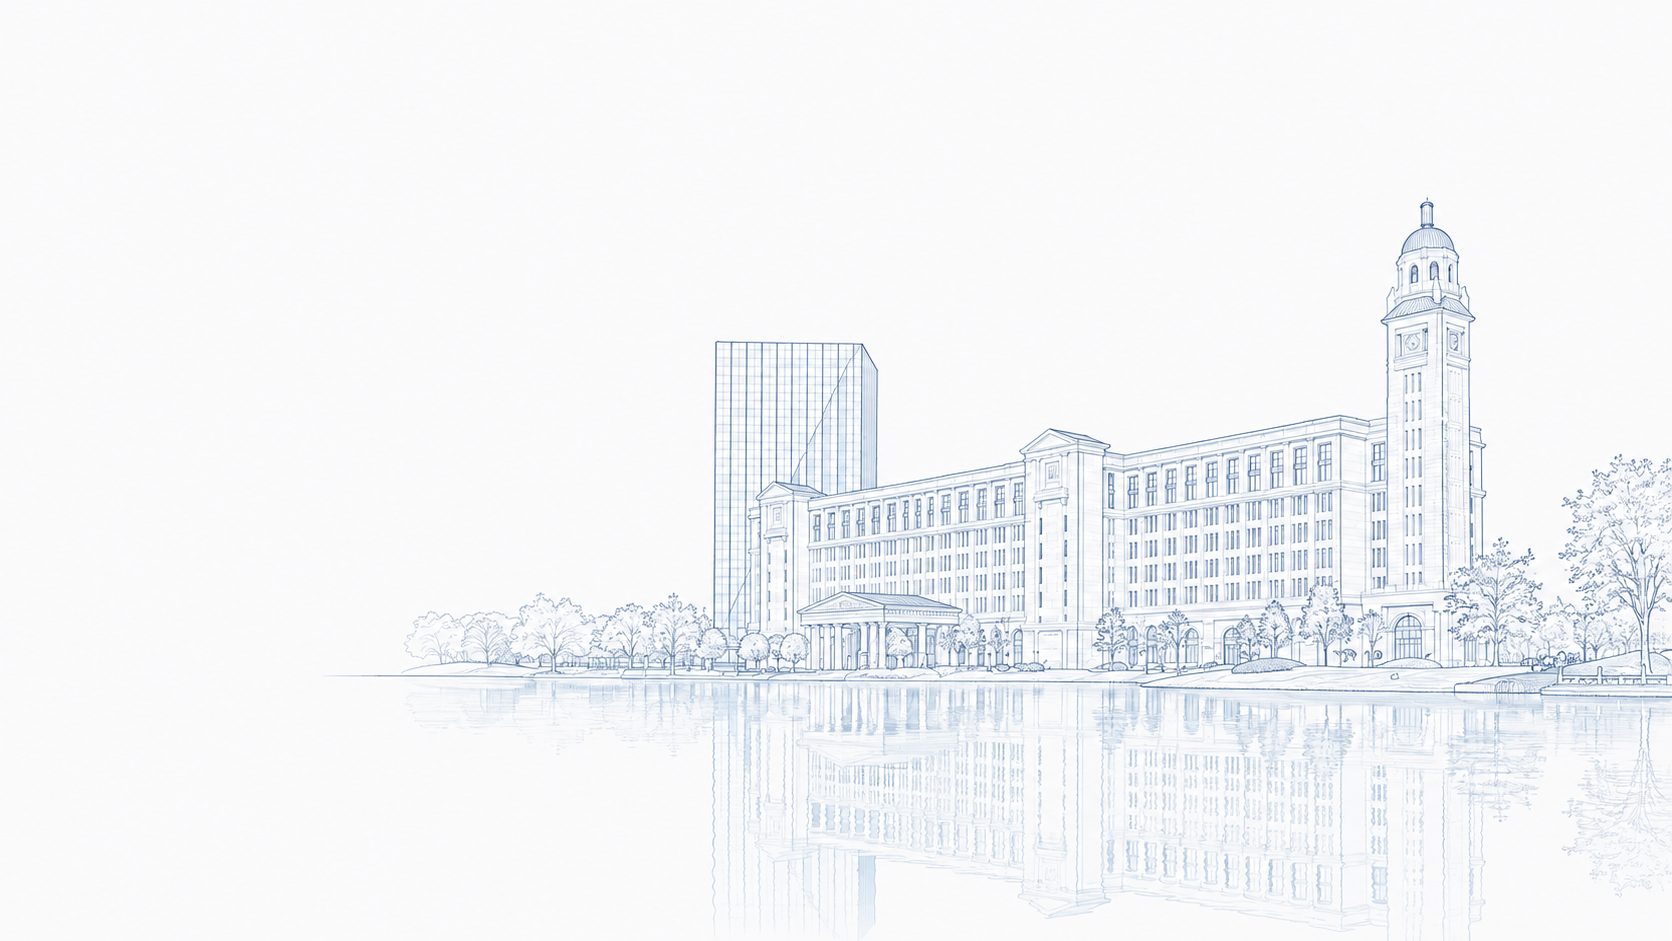
\includegraphics[width=\paperwidth,height=\paperheight]{cover_background.png}};
\node[anchor=north west,text=accent,font=\songti\bfseries]
 at ([xshift=.065\paperwidth,yshift=-.24\paperheight]current page.north west)
 {\fontsize{29}{36}\selectfont 谢谢};
\draw[accent,line width=1.3pt] ([xshift=.065\paperwidth,yshift=-.43\paperheight]current page.north west)--([xshift=.43\paperwidth,yshift=-.43\paperheight]current page.north west);
\draw[accent,line width=3.4pt] ([xshift=.065\paperwidth,yshift=-.43\paperheight]current page.north west)--([xshift=.14\paperwidth,yshift=-.43\paperheight]current page.north west);
\node[anchor=north west,text=accent,font=\songti\large]
 at ([xshift=.065\paperwidth,yshift=-.465\paperheight]current page.north west) {欢迎讨论};
\end{tikzpicture}
\end{frame}
\end{document}
